% Neurocomputing submission manuscript adapted to the CAS double-column template.
\documentclass[a4paper,fleqn]{cas-dc}

\usepackage{amsmath}
\usepackage{amssymb}
\usepackage{booktabs}
\usepackage{multirow}
\usepackage{graphicx}
\usepackage{pgfplots}
\usepackage{subcaption}
\usepackage{algorithm}
\usepackage{algorithmic}
\usepackage{listings}
\usepackage[numbers,sort&compress]{natbib}
\usepackage{placeins}
\usepackage{needspace}
\usepackage{balance}
\usetikzlibrary{arrows.meta}
\pgfplotsset{compat=1.18}
% Moderate float separation; preserve body font and page geometry.
\setlength{\textfloatsep}{12pt plus 2pt minus 2pt}
\setlength{\dbltextfloatsep}{12pt plus 2pt minus 2pt}
\setlength{\floatsep}{10pt plus 2pt minus 2pt}
\setlength{\dblfloatsep}{10pt plus 2pt minus 2pt}
% Keep justified paragraphs readable while allowing legal line breaks in long
% technical terms.  Blocking hyphenation creates overfull boxes in two-column
% mode, especially in headings and dataset names.
\hyphenpenalty=250
\exhyphenpenalty=50
% Allow a column break after a hyphenated line instead of leaving a large gap.
\brokenpenalty=100
\tolerance=2000
\emergencystretch=1.5em

% PDF metadata for the manuscript record.
\hypersetup{
  pdftitle={CALIPER: A Locality-Aware Collaborative Local--Cloud Architecture for Retrieval-Augmented Generation},
  pdfauthor={Yang Gao, Chao Liao, Xinteng Zhou, Zeyuan Hu, Bingde Hu, Mingli Song},
  pdfsubject={Retrieval-Augmented Generation}
}
% The CAS class rewrites author and subject during \maketitle; reapply the
% manuscript metadata after that command while keeping the configuration here.
\AddToHook{cmd/maketitle/after}{%
  \hypersetup{
    pdftitle={CALIPER: A Locality-Aware Collaborative Local--Cloud Architecture for Retrieval-Augmented Generation},
    pdfauthor={Yang Gao, Chao Liao, Xinteng Zhou, Zeyuan Hu, Bingde Hu, Mingli Song},
    pdfsubject={Retrieval-Augmented Generation}%
  }%
}

\begin{document}
\let\WriteBookmarks\relax
% Suppress the empty ORCID footnote until identifiers are supplied.
\renewcommand{\printorcid}{}
\def\floatpagepagefraction{1}
\def\textpagefraction{.001}

\shorttitle{CALIPER: Local--Cloud RAG}
\shortauthors{Y. Gao et al.}

\title[mode = title]{CALIPER: A Locality-Aware Collaborative Local--Cloud Architecture for Retrieval-Augmented Generation}

% Author order retained; affiliations updated per author confirmation on 2026-09-23.
\author[inst1]{Yang Gao}
\fnmark[1]
\ead{roygao@zju.edu.cn}
\author[inst2]{Chao Liao}
\fnmark[1]
\ead{liaochao@zju.edu.cn}
\author[inst2]{Xinteng Zhou}
\ead{xintengzhou@zju.edu.cn}
\author[inst3,inst4]{Zeyuan Hu}
\ead{huzeyuan@zj.chinamobile.com}
\author[inst3]{Bingde Hu}
\cormark[1]
\ead{tonyhu@zju.edu.cn}
\author[inst3]{Mingli Song}
\ead{brooksong@zju.edu.cn}

\affiliation[inst1]{organization={Zhejiang Polytechnic University of Mechanical and Electrical Engineering}, country={China}}
\affiliation[inst2]{organization={College of Software Technology, Zhejiang University}, city={Hangzhou}, country={China}}
\affiliation[inst3]{organization={College of Computer Science, Zhejiang University}, city={Hangzhou}, country={China}}
\affiliation[inst4]{organization={China Mobile (Zhejiang) Research \& Innovation Institute}, country={China}}
\fntext[1]{These authors contributed equally to this work.}
\cortext[1]{Corresponding author.}

\begin{abstract}
Retrieval-augmented generation (RAG) grounds answers in external knowledge, addressing the limitations of relying solely on parametric knowledge in knowledge-intensive question answering. Cloud RAG uses powerful language models to process retrieved evidence, but requires transferring local evidence to the cloud and incurs remote processing and generation overhead. Fully local execution avoids evidence transfer but leaves evidence interpretation and answer generation to a less capable local model. The central challenge is to obtain useful cloud assistance without transferring retrieved evidence while controlling the overhead of collaboration. We propose CALIPER, a local--cloud collaborative RAG framework that separates these responsibilities: the cloud generates guidance from the question alone, while the local model combines that guidance with retrieved evidence to answer. Because the collaboration still depends on effective local evidence, CALIPER selects a source-specialized retriever according to the predicted query source. An optional execution classifier bypasses collaboration for queries predicted to be locally answerable and sends the remaining queries through the collaborative path. Experiments show that CALIPER improves answer quality over the local-model baseline and narrows the gap to the cloud reference. In the latency evaluation, it reduces estimated end-to-end answering latency relative to the two-stage cloud reasoning reference. The optional classifier further reduces estimated answering latency at some cost in answer quality. These results support question-guided collaboration as a way to improve the answer-quality--latency trade-off.
\end{abstract}

\begin{keywords}
Retrieval-Augmented Generation \sep Local--Cloud Collaboration \sep Data Locality \sep Multi-Hop Question Answering \sep Adaptive Retrieval \sep Large Language Models
\end{keywords}

\maketitle

\section{Introduction}
Retrieval-augmented generation (RAG) uses external knowledge to ground language-model answers, reducing reliance on information stored in model parameters \cite{lewis2020retrieval}. For knowledge-intensive questions, retrieval supplies relevant evidence, while the answering model must interpret that evidence and connect it to the question. Using a powerful cloud model is one way to support this process, but it also determines where the evidence is processed.

In a conventional cloud RAG workflow, retrieved passages accompany the question to the remote model. When these passages contain internal or sensitive knowledge, this transfer expands the information available outside the local infrastructure. In deployments that require evidence to remain local, sending passages is therefore not simply a performance choice: it conflicts with the evidence-access boundary. Remote evidence processing and answer generation also introduce response-time overhead. Keeping the entire workflow local avoids evidence transfer, but leaves a smaller model responsible for both interpreting evidence and producing the answer. The central challenge is thus to obtain useful cloud assistance without transferring retrieved evidence to the cloud, while controlling the additional latency of collaboration.

Existing approaches offer several forms of local--cloud cooperation. Model cascades and adaptive routing select models or workflows according to query requirements and computational cost \cite{chen2023frugalgpt,ong2025routellm,jeong2024adaptive}. Other approaches rewrite requests before cloud submission, align cloud guidance with personalized local tasks, or aggregate outputs generated from separately held documents \cite{siyan2025papillon,zhang2025lsrp,liu2025dragon}. These approaches establish alternatives to placing the entire answering task on one side. Against this background, we ask how question-only cloud guidance can complement source-adapted local retrieval, and when such collaboration is worth invoking.

Two practical problems remain. First, cloud guidance cannot substitute for evidence that local retrieval fails to supply. Dense retrieval and reranking address evidence selection \cite{xiao2024c,nogueira2019passage}, but questions from different sources can differ in structure and evidence needs. A specialized retriever must therefore be selected without access to the question's source label at inference. Second, applying cloud assistance to every query adds calls even when the local model could already answer. Evidence adaptation and collaboration selection consequently require distinct decisions: which evidence model to use, and whether cloud assistance is needed.

We propose CALIPER, a locality-aware collaborative local--cloud RAG framework. As illustrated in Figure~\ref{fig1}, the cloud generates reasoning instructions from the question alone, while the local model combines them with retrieved evidence to answer. A source router supports evidence adaptation, and a separate optional execution classifier avoids unnecessary collaboration. The framework thus addresses the three needs together: useful cloud assistance without evidence transfer, source-adapted retrieval, and on-demand collaboration.

\begin{figure}[pos=t]
\centering
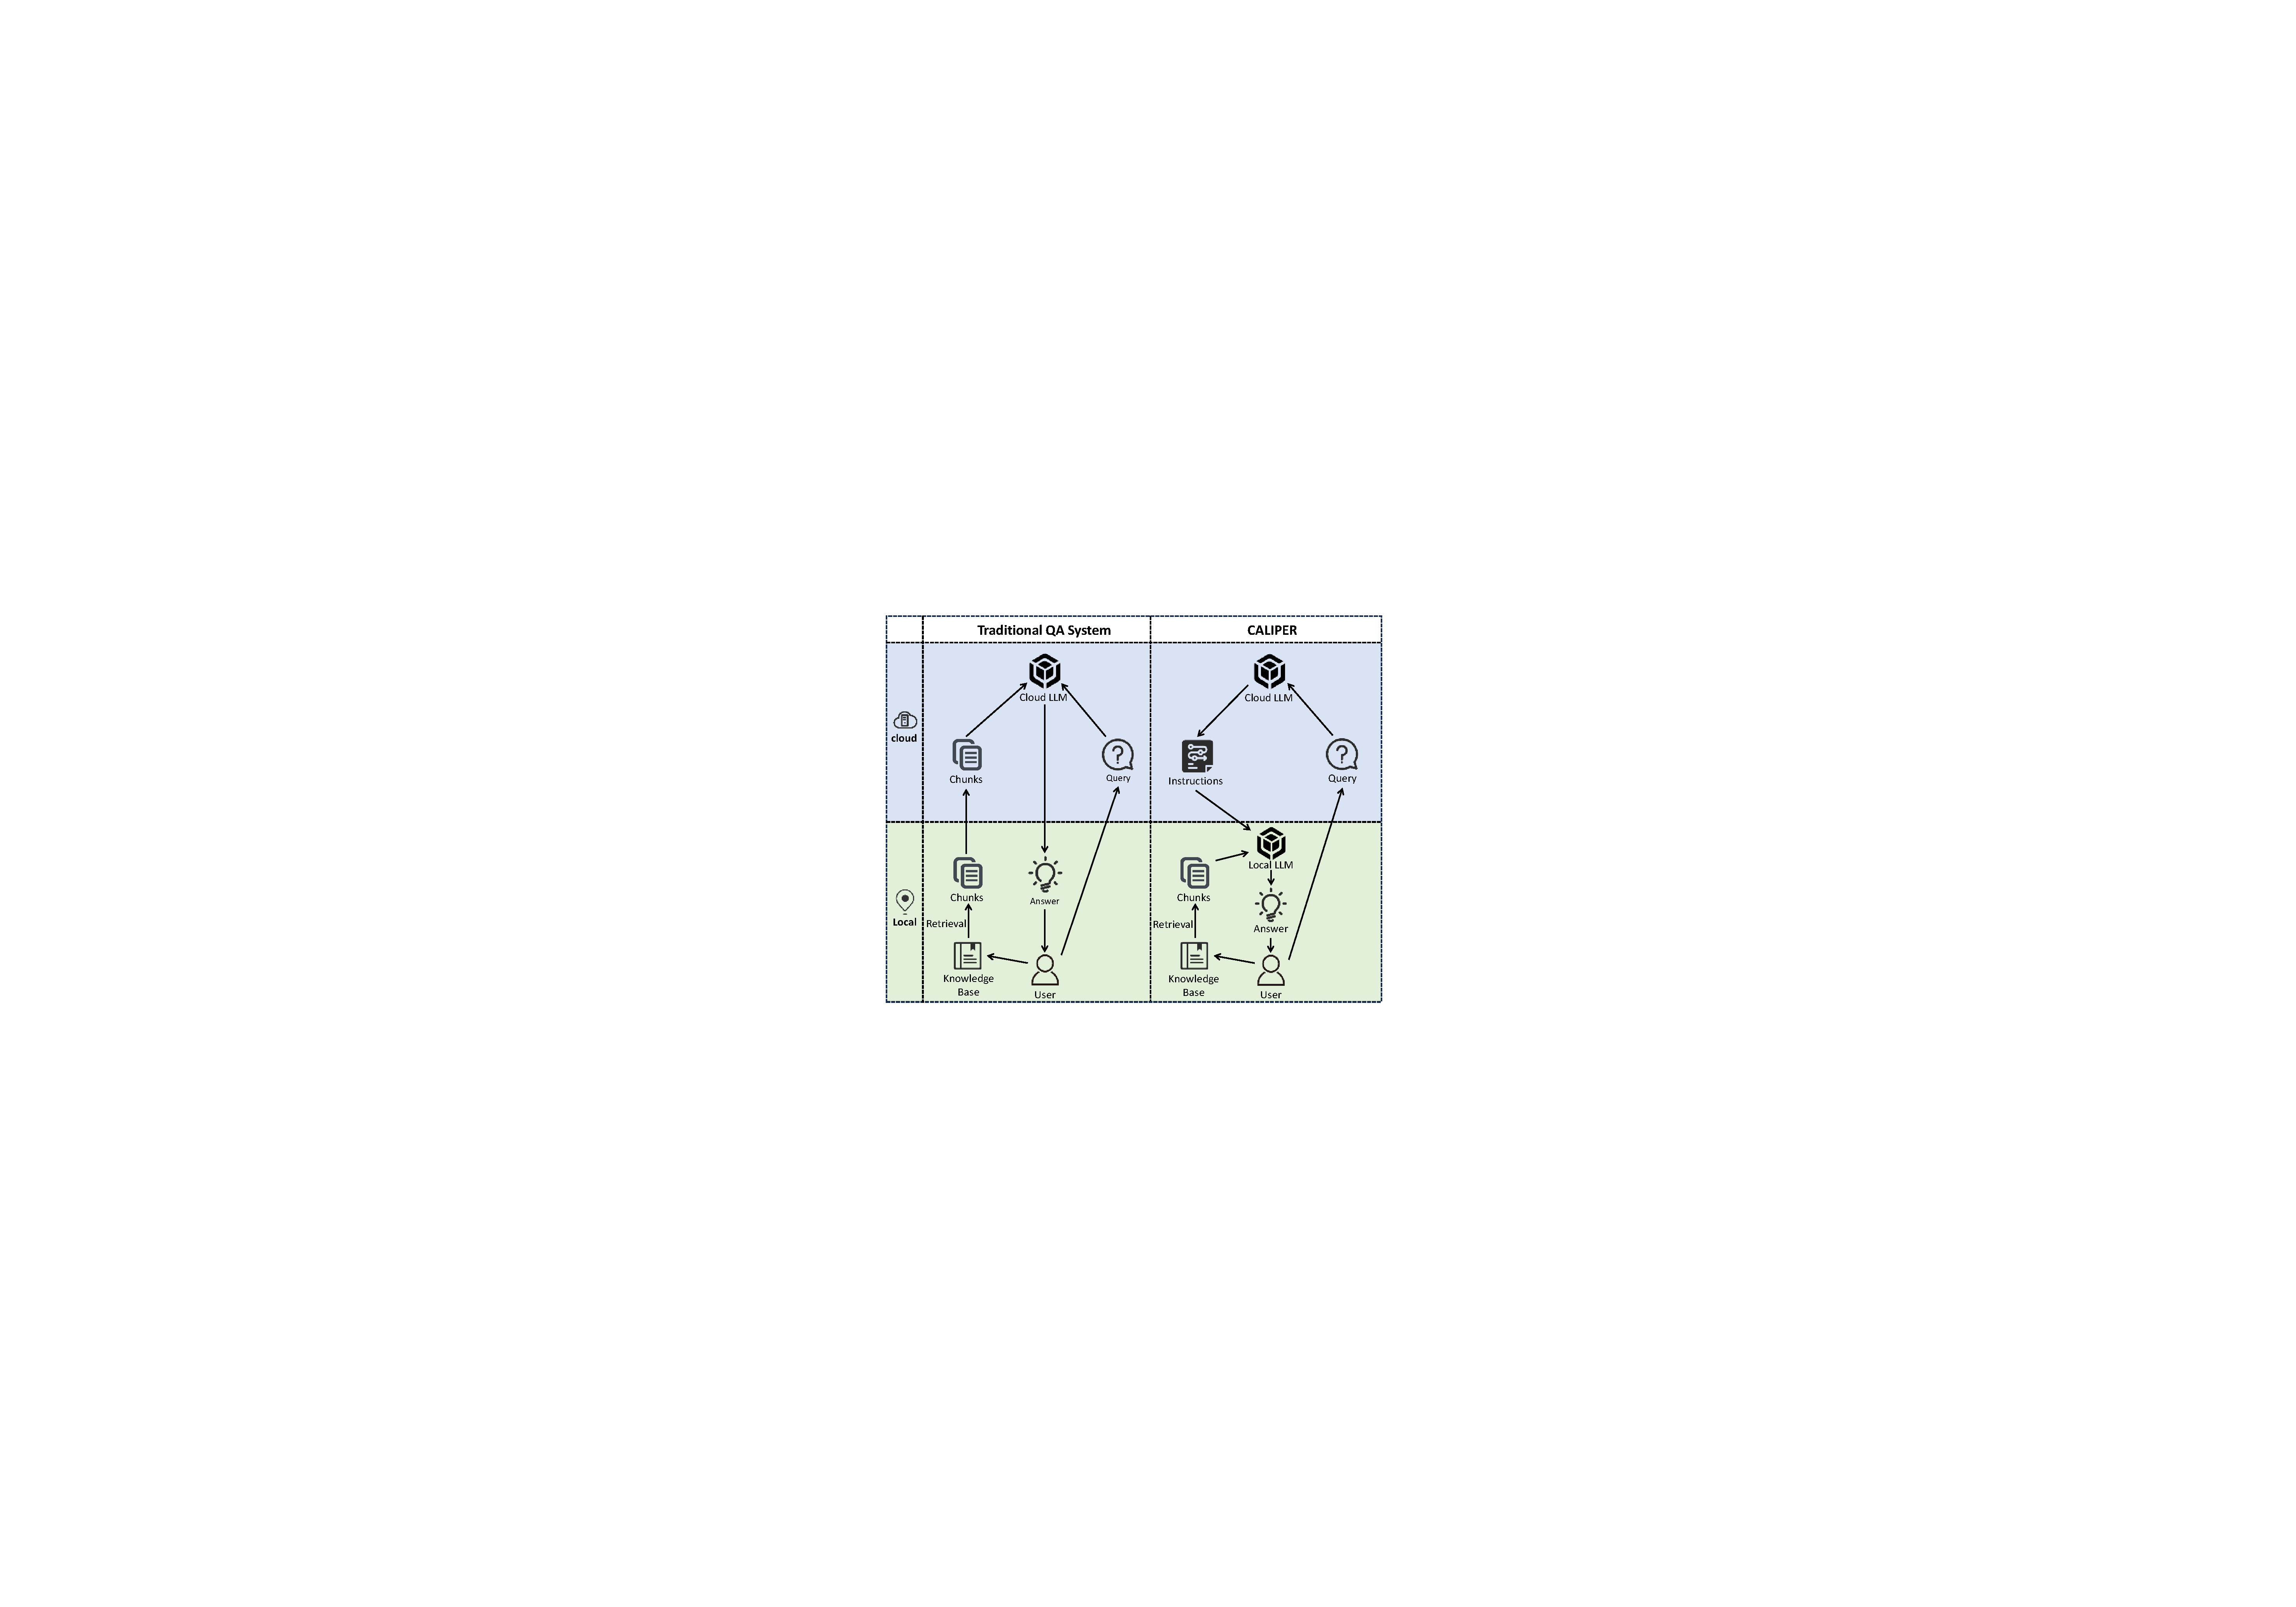
\includegraphics[width=0.9\columnwidth]{motivation}
\caption{Data flow in cloud RAG (left) and CALIPER (right). CALIPER sends the query for cloud guidance while keeping retrieved evidence local.}
\label{fig1}
\end{figure}

Our contributions are:
\begin{itemize}
\item \textbf{Evidence-local collaborative reasoning:} We develop a collaborative RAG workflow in which the cloud receives only the question and returns guidance that the local model uses with retrieved evidence to reason and answer. This makes cloud assistance available without transferring retrieved evidence to the cloud. Experiments show improved answer quality over the local-model baseline and, in a separate latency evaluation, lower estimated answering latency than the two-stage cloud reasoning reference.
\item \textbf{Source-aware specialized retrieval:} We combine separately fine-tuned retriever--reranker pairs with a lightweight source router, making evidence adaptation a per-query decision rather than requiring a manually supplied source label. The design connects source-specific training to local evidence selection while keeping source selection separate from execution selection; comparisons on known benchmark sources assess its retrieval and answering effects without assuming specialization helps every dataset.
\item \textbf{Lightweight classification for on-demand collaboration:} We introduce an execution classifier that selects local-only or collaborative answering according to predicted local answerability. Independent of the source router, it addresses whether cloud assistance is needed rather than which retriever to use. This avoids applying the same collaboration overhead to every query and, at the evaluated operating point, further reduces estimated answering latency with a corresponding answer-quality cost.
\end{itemize}


\section{Related Work}

\subsection{Local--Cloud Collaboration and Evidence Locality}
Local--cloud collaboration determines both where computation runs and what information crosses the boundary \cite{teerapittayanon2017distributed}. In RAG, generated outputs can expose retrieved content \cite{zeng2024good}. PRAG and RemoteRAG address information exposure through multi-party computation and distance-based differential privacy, respectively \cite{zyskind2024don,cheng2025remoterag}.

Other approaches organize cooperation through the information exchanged between models. PAPILLON optimizes local prompts to construct privacy-conscious cloud requests and combine cloud responses with the original user request \cite{siyan2025papillon}. LSRP aligns cloud guidance with personalized local tasks through retrieval of task-specific leader strategies and preference optimization using small-model feedback \cite{zhang2025lsrp}. DRAGON keeps document processing on the respective cloud and device sides, aggregating token-level outputs with speculative aggregation to reduce synchronization overhead \cite{liu2025dragon}.

CALIPER shares with this line of work the use of cloud assistance for local answering, particularly with LSRP. LSRP also uses cloud-generated guidance with private device-side processing, so query-only cloud input is not itself our novelty claim. LSRP focuses on personalized cloud--device collaboration through task-specific leader-strategy retrieval and small-model-feedback alignment. CALIPER addresses a different systems setting: multi-hop evidence-grounded QA with source-specialized retriever--reranker routing, an answerability-based execution gate, and a quality--latency evaluation. Its contribution is the composition and evaluation of these evidence-local decisions, rather than cloud guidance alone.

\subsection{Retrieval Adaptation for Evidence Quality}
Evidence quality can be improved through relevance modeling or evidence organization. Dense retrieval and passage reranking learn which candidates best match a query \cite{xiao2024c,nogueira2019passage}; LM-supervised reranking further addresses passage quality and context length \cite{zhai2025rag}. Structured retrieval instead exploits connections among evidence units. Graph-based methods, including HippoRAG, organize entities, relations, or passages for traversal \cite{he2024g,gutierrez2024hipporag,fang2024trace}; chunk-interaction, topic-linked, and relation-enhanced approaches use complementary structures for multi-hop evidence discovery \cite{guo2025leveraging,chen2026tgrag,li2025recot}.

These routes primarily change how a retrieval model scores or connects evidence. CALIPER adds a different selection decision: which source-specialized retriever--reranker pair should process an incoming question? It combines source-specific fine-tuning with query-based model selection, and evaluates adaptation among known benchmark sources rather than superiority over structured retrieval or generalization to unseen domains.

\subsection{Adaptive Execution and Compute Allocation}
Adaptive execution methods differ in the decision they control. Model cascades and RouteLLM select among models with different capabilities and costs \cite{li2021cascadebert,chen2023frugalgpt,ong2025routellm}. Adaptive-RAG selects no-retrieval, single-step, or iterative workflows based on predicted question complexity \cite{jeong2024adaptive}. Retrieval-control methods instead decide whether further evidence is needed: Self-RAG learns retrieval and self-critique, CRAG uses evidence evaluation to trigger corrective retrieval, and adaptive iterative retrieval feeds generation feedback into subsequent retrieval \cite{asai2024self,yan2024corrective,han2025adaptive}.

CALIPER instead decides whether to invoke question-only cloud guidance, using predicted answerability by the tested local model rather than a model-independent notion of question difficulty. This is separate from choosing a retriever or deciding whether to retrieve more evidence, and is evaluated as an answer-quality--latency trade-off.

\section{Method}
CALIPER takes a question and its supplied candidate contexts as input. It separates cloud question guidance from local evidence-grounded answering. Figure~\ref{fig2} shows source-routed retrieval, collaborative reasoning, and optional execution classification. The search space is restricted to each question's supplied contexts or paragraphs, rather than the full Wikipedia corpus. Retrieval, reranking, and generation operate on sentence-level text units extracted from these contexts; reported quality and costs are conditional on this search space.

\begin{figure*}[pos=t]
\centering
% Use the author-selected workflow PDF with its existing crop box.
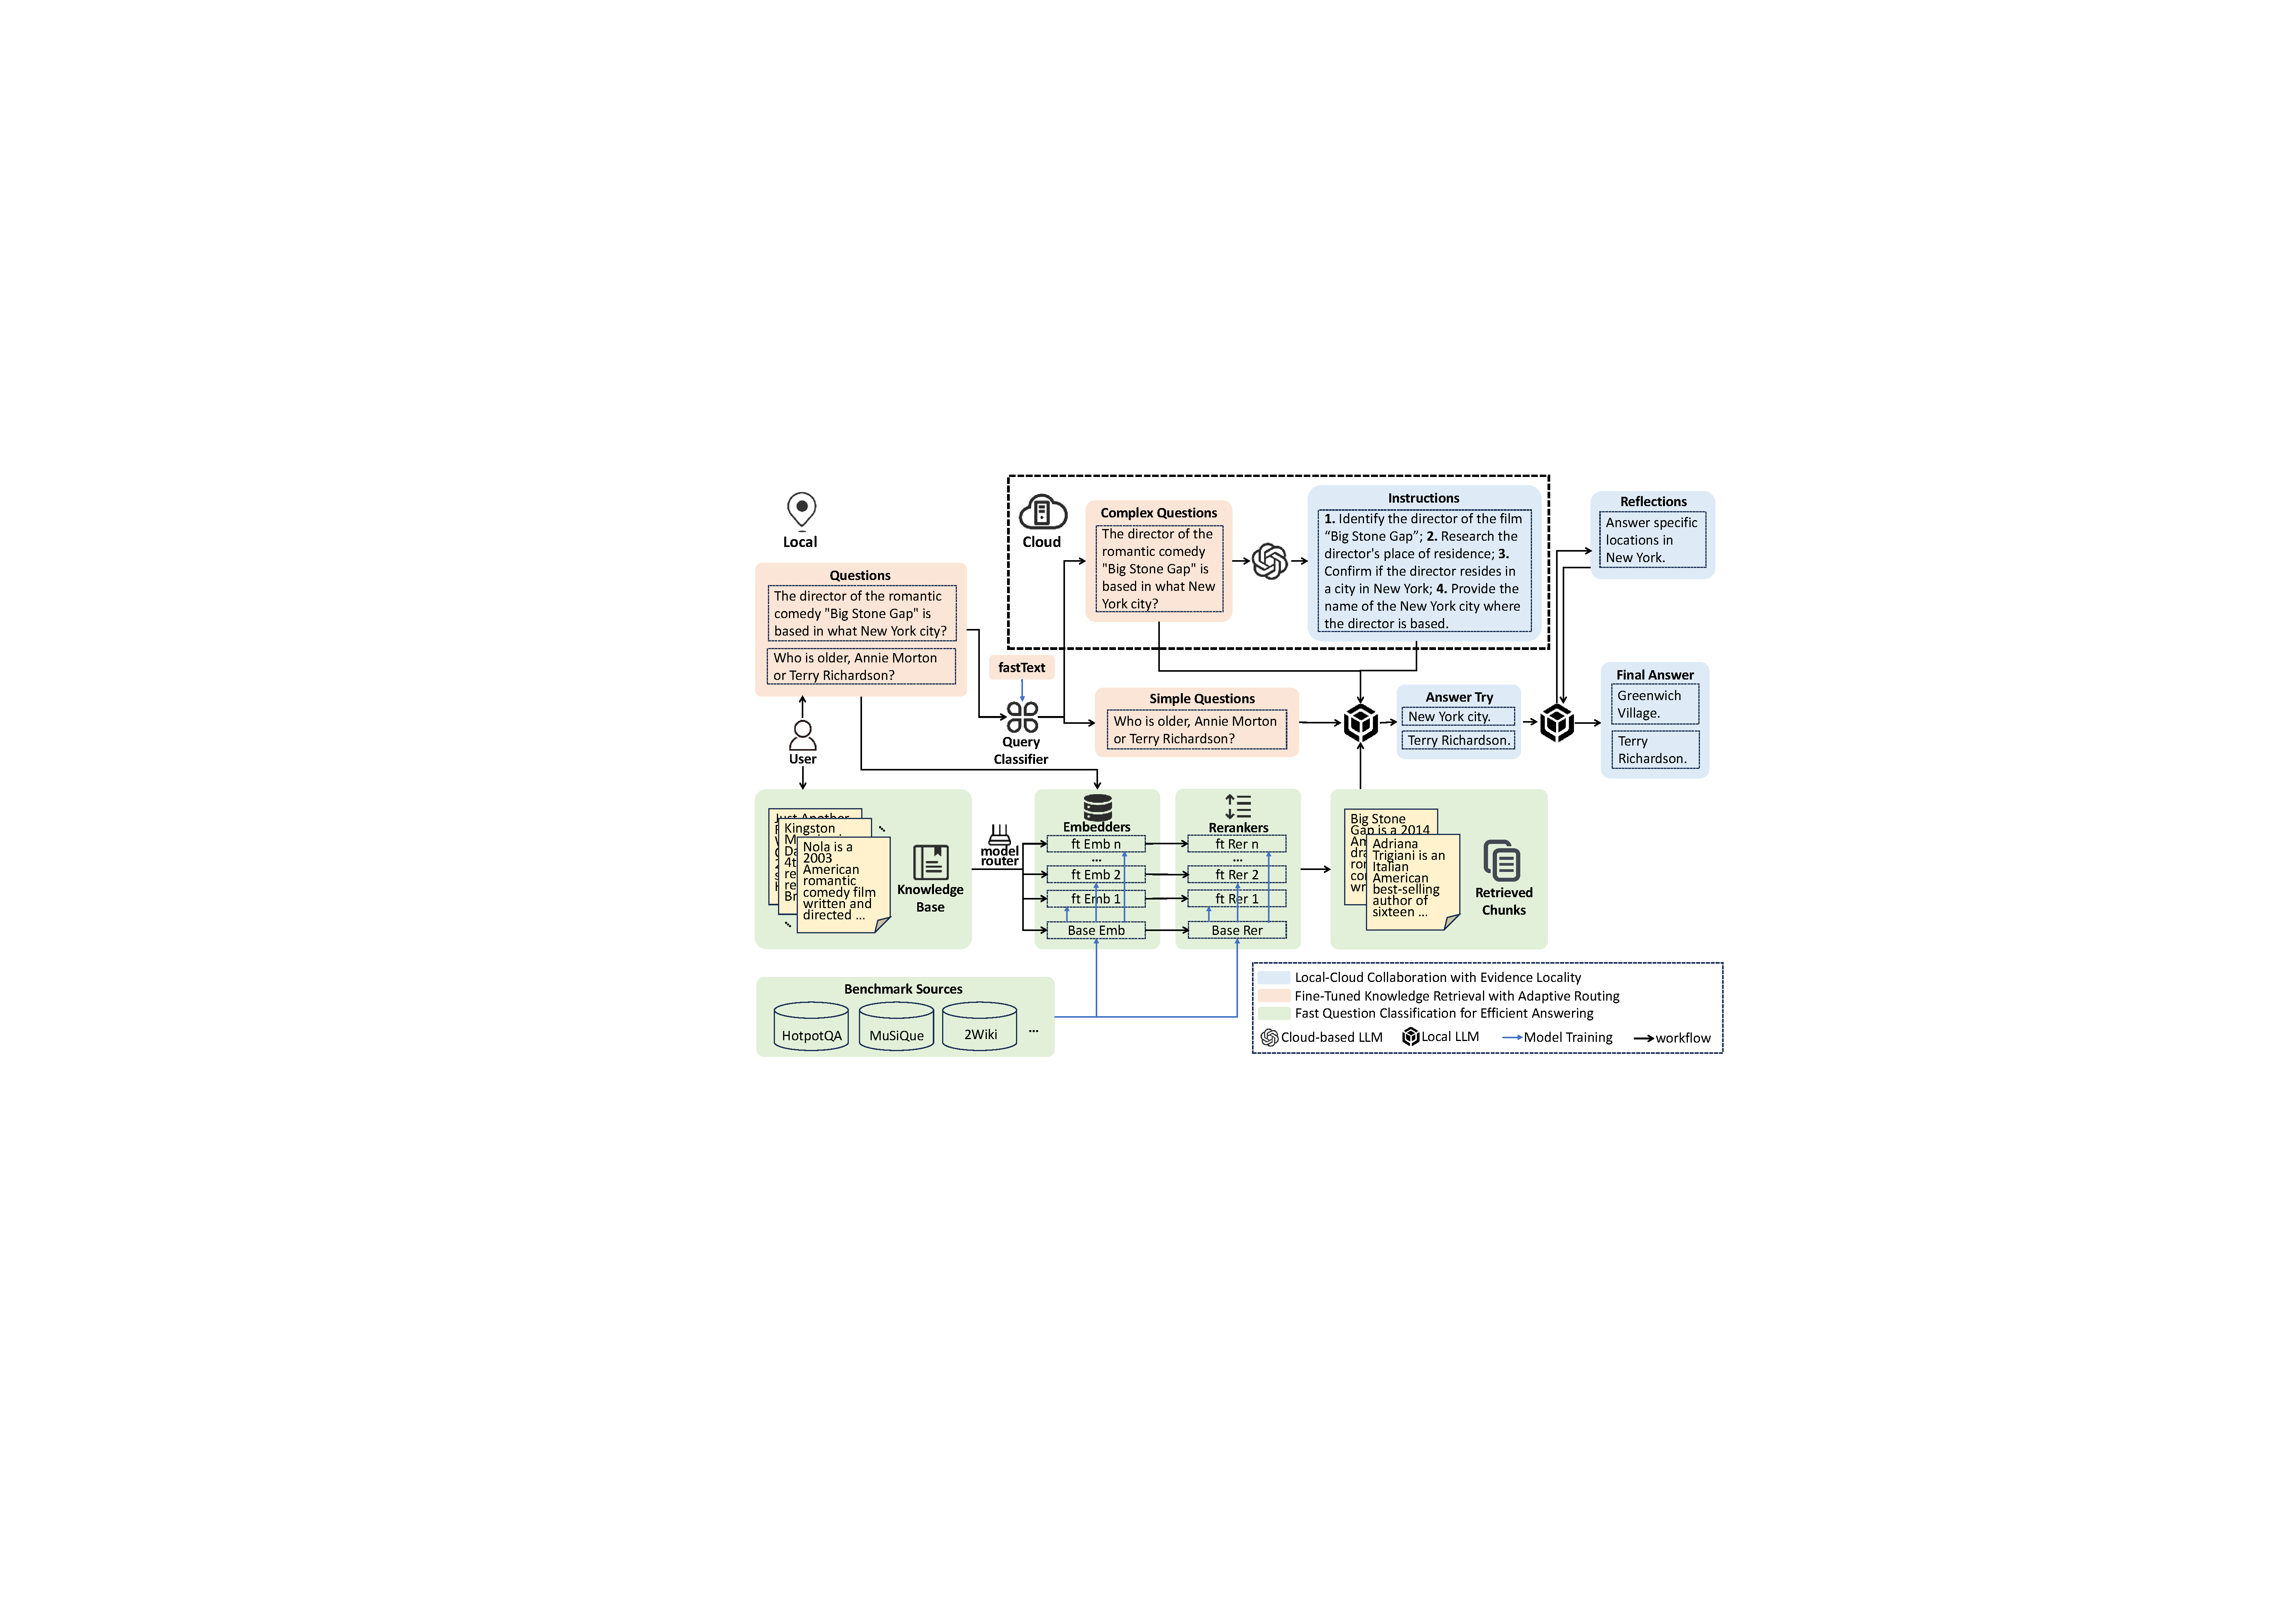
\includegraphics[width=\textwidth]{workflow.pdf}
\caption{CALIPER architecture. The cloud model receives only the question and returns guidance; retrieval and answering remain local. Source routing and the optional execution classifier serve separate decisions; the query classifier denotes the CALIPER+clf variant.}
\label{fig2}
\end{figure*}

\subsection{Local--Cloud Synergy with Retrieved-Evidence Locality}
The cloud offers question-level guidance but cannot verify it against local passages it has not received. CALIPER therefore keeps retrieval, evidence interpretation, and final answer generation local, making assistance available within the evidence-locality boundary.

Let \(q\) denote a question, \(\mathcal{D}(q)=\{d_i\}_{i=1}^{N_q}\) its candidate sentence-level evidence units, and \(\hat{s}=\rho(q)\) the source label predicted by the router.

% Permit a column break before this display instead of moving its lead-in
% paragraph with the equation and leaving the previous column unfilled.
\begingroup
\predisplaypenalty=0
The source router selects the embedder and reranker. The embedder scores question--unit similarity; the cross-encoder then reranks dense candidates using query--unit pairs, as defined in Eq.~\eqref{eq:retrieval}.
\begin{equation}\label{eq:retrieval}
\begin{aligned}
\mathcal{C}_K(q)&=\operatorname{TopK}_{d\in\mathcal{D}(q)}\,\operatorname{sim}_{\hat{s}}(q,d),\\
R(q)&=\operatorname{Topk}_{d\in\mathcal{C}_K(q)}\,r_{\hat{s}}(q,d),
\end{aligned}
\end{equation}
where \(\operatorname{sim}_{\hat{s}}(q,d)=\cos\langle Emb_{\hat{s}}(q),Emb_{\hat{s}}(d)\rangle\), \(r_{\hat{s}}(q,d)\) is the scalar cross-encoder score for the query--unit pair, and \(Emb_{\hat{s}}\) and \(r_{\hat{s}}\) denote the source-selected embedder and reranker. \(\operatorname{TopK}\) returns the ranked dense-retrieval candidate units, and \(\operatorname{Topk}\) returns the final \(k\) reranked units; \(K\) and \(k\) are the candidate-pool and final-context sizes, respectively.
\par\endgroup

For CALIPER core, the routed context above is used for collaborative generation. In the evaluated CALIPER+clf composition, the operational-difficulty classifier selects frozen local two-stage baseline answers for queries predicted as easy and current core answers for the remainder; the easy branch does not rerun the source router. Operationally, this gate is applied before the collaborative branch: an easy query exits to the frozen local two-stage answer, whereas a hard query proceeds through source-routed retrieval, question-only cloud guidance, and local evidence-grounded generation.

For collaborative inference, the cloud model generates natural-language guidance from the question and its parametric knowledge. The guidance may contain question decomposition, entities or relations to connect, a reasoning sequence, or model-inferred candidate answers, but it has not been verified against local evidence.

The local model receives the question, retrieved evidence units, and guidance together. The prompt presents the guidance as a reference rather than an authoritative answer, and asks the local model to reason beyond the hints using the local evidence. The cloud output is therefore used as input to local evidence interpretation and answer generation, not returned directly as the final answer. Local generation has two stages: the model first produces a reasoning trace \(h\) using the evidence and guidance, then extracts a concise answer from that trace and the question, as formalized in Eqs.~\eqref{eq:guidance}--\eqref{eq:local-generation}:
\begin{equation}\label{eq:guidance}
ins=C_{ins}(q),
\end{equation}
\begin{equation}\label{eq:local-generation}
h=L_{exe}(\operatorname{Pack}(R,q,ins)),\qquad a_0=L_{extract}(h,q),
\end{equation}
where \(\operatorname{Pack}\) assembles the retrieved evidence units, question, and instruction into the local prompt; \(L_{exe}\), \(L_{extract}\), and the reflection operations below are local-model operations, while \(C_{ins}\) is the cloud instruction call.

Guidance provides a question-specific starting point for connecting evidence rather than a generic procedure. Its value depends on the guidance, the retrieved evidence, and the local model's ability to use both; it does not guarantee correct guidance or reliable detection of erroneous hints. The ablation study evaluates its contribution to answer quality.

Reflection is an optional post-generation enhancement rather than part of CALIPER core. A local evaluator checks the temporary answer; if revision is requested, a local corrector produces feedback and regenerates the answer, for at most three revision attempts. The process stops when the evaluator accepts the answer or the cap is reached. Unlike Reflexion's cross-trial verbal feedback stored in episodic memory \cite{shinn2023reflexion}, this procedure revises only the current answer, without cross-trial memory or model updates. The revision functions and stopping rule are given in Eqs.~\eqref{eq:reflection-functions}--\eqref{eq:reflection-update}.
\begin{equation}\label{eq:reflection-functions}
\begin{aligned}
u_j&=L_{ref}(h,R,q,a_j),\\
f(a_j)&=L_{extract}(h,q,u_j).
\end{aligned}
\end{equation}
\begin{equation}\label{eq:reflection-update}
\begin{aligned}
a_{j+1}&=
\begin{cases}
f(a_j), & \begin{aligned}[t]
          &L_{eval}(q,R,h,a_j)=0\\
          &\mathrm{and}\ j<3,
          \end{aligned}\\
a_j, & \mathrm{otherwise},
\end{cases}
\end{aligned}
\end{equation}
for \(j=0,1,2\), where \(L_{ref}\) returns a revision instruction and \(L_{eval}(q,R,h,a_j)\) returns 1 when the answer is accepted and 0 when it requests revision. The final answer is the first accepted \(a_j\), or \(a_3\) if no attempt is accepted.

Implementation-specific evaluator settings and the 200-question reflection audit are reported in the Supplementary Configuration Notes. The full-set V0 artifacts retain final predictions but not complete intermediate traces, so iteration distributions are not inferred from them.

The collaborative cloud call receives the raw question only, not the local knowledge base, retrieved passages, passage embeddings, source labels, local predictions, or classifier scores. Queries and returned guidance may still reveal sensitive information; deployment limitations are discussed in Section~5. Table~\ref{time} follows the separate latency-estimation protocol in Section~4.1, which also specifies the different payload of the cloud reference.

\subsection{Fine-Tuned Retrieval with Source Routing}
Cloud guidance cannot replace missing local evidence. Source-specialized retrieval addresses evidence selection, but requires choosing a model without the true source label. A lightweight \textit{fastText} router \cite{joulin2017bag} predicts the benchmark-source label and selects the corresponding embedder--reranker pair. These labels are domain proxies, not evidence of deployment-time domain generalization.

We fit the router only on the source training corpora, keeping evaluated questions outside model fitting. Labeled questions from the three benchmark sources form the router-training pool in Eq.~\eqref{eq:router-pool}
\begin{equation}\label{eq:router-pool}
D_{\rho}=\{(q_i,s_i)\}_{i=1}^{N_{\rho}},\qquad s_i\in\{1,\ldots,H\},
\end{equation}
where \(s_i\) is the dataset-source label. The pool is split by normalized question text, with evaluation overlap excluded; split counts and construction details are provided in the Supplementary Configuration Notes. The experiments cover the three known benchmark sources, with BASE as the non-specialized reference.

MuSiQue uses two positive-pool constructions: first-position uses the first sentence of each supporting paragraph, whereas full-train uses all supporting-paragraph sentences. Detailed candidate-pool construction and training settings are given in the Supplementary Configuration Notes.

The embedder aims to maximize the similarity between \(q_n\) and \(d_n^+\), while minimizing it with respect to \(d_{n,m}^-\). Training uses one positive and seven sampled negatives per query, so \(M=7\); \(N_{\mathrm{train}}\) is the number of training query groups. The score function and InfoNCE objective are given in Eqs.~\eqref{eq:embed-score}--\eqref{eq:embed-loss}.
\begin{equation}\label{eq:embed-score}
g(x,y):=\exp\left(\cos\langle Emb(x),Emb(y)\rangle/\tau\right),
\end{equation}
\begin{equation}\label{eq:embed-loss}
\mathcal{L}_{emb} = -\sum_{n=1}^{N_{\mathrm{train}}} \log \frac{g(q_n, d_n^+)}{g(q_n, d_n^+) + \sum_{m=1}^{M} g(q_n, d_{n,m}^-)},
\end{equation}
where \(\tau\) denotes a temperature parameter that controls the sharpness of the softmax distribution.

Following embedding retrieval, the cross-encoder produces a scalar relevance logit \(r_{\theta}(q,d)\) for a query--unit pair and scores one positive unit against sampled negatives using the groupwise cross-entropy in Eq.~\eqref{eq:reranker-loss}:
\begin{equation}\label{eq:reranker-loss}
\resizebox{0.92\columnwidth}{!}{$\displaystyle
\mathcal{L}_{\text{rer}}=-\sum_{n=1}^{N_{\mathrm{train}}}\log
\frac{\exp r_{\theta}(q_n,d_n^+)}{\exp r_{\theta}(q_n,d_n^+)+\sum_{m=1}^{M}\exp r_{\theta}(q_n,d_{n,m}^-)}.
$}
\end{equation}

Unless noted otherwise, generation uses the top five reranked sentence-level units directly, without expanding them to parent paragraphs. For MuSiQue evaluation questions, BASE top-three units are merged and deduplicated by lowercased, whitespace-normalized text. The routed row of Table~\ref{retrieval} excludes this additional BASE stream. Segmentation rules appear in the Supplementary Configuration Notes.

All retrievers in Table~\ref{retrieval} share the \textit{bge-base-en-v1.5} embedder and \textit{bge-reranker-large} initialization backbones \cite{xiao2024c}, but differ in fine-tuning data and final weights. FT-SEP trains source-specific pairs and is the source-known reference, whereas FT-MER is a system-level merged-data comparator. MuSiQue uses a source-specific first-position embedder with a merged-data reranker for FT-MER; its FT-SEP retrieval-only row uses full-train, while the routed and end-to-end rows use first-position. These configurations make Table~\ref{retrieval} a system-level comparison rather than a single-factor routing ablation. Checkpoint mappings are retained in the Supplementary Configuration Notes. The embedding--reranking pipeline follows established passage-search practice \cite{khattab2020colbert,nogueira2019passage}.

\subsection{Fast Question Classification for Efficient Answering}
A separate fastText execution classifier estimates local answerability to bypass selected collaborative calls. Source routing chooses an evidence model; execution classification decides whether to use cloud guidance. A false easy prediction can withhold useful assistance, making this a quality--cost decision. Difficulty is operational and model-dependent, not an intrinsic property of the question.

A query is labeled easy only when all three frozen local baseline runs contain the normalized gold answer; otherwise it is labeled hard, as defined in Eq.~\eqref{eq:classifier-label}:
\begin{equation}\label{eq:classifier-label}
y_i=\left\{\begin{array}{ll}
    \text{easy}, & \prod_{j=1}^{3} hit(L^{(j)}_{local}(R_i,q_i))=1, \\
    \text{hard}, & \text{otherwise}.
\end{array}\right.
\end{equation}
The classifier estimates \(p_{easy}=clf(q_i)\). Local-only inference is used when \(p_{easy}\ge t\); otherwise the query is routed to collaborative inference. This model-derived labeling introduces circularity and limits transfer to other model families.

We freeze dataset-specific thresholds \(t_{\mathrm{HP}}=0.974\), \(t_{\mathrm{Mu}}=0.978\), and \(t_{\mathrm{2Wiki}}=0.977\). Each is the smallest 0.001-grid threshold with at most 10\% false negatives among truly hard questions in its overlap-free validation pool. Known benchmark-pool identity selects the threshold before source routing; the router's prediction selects retrieval weights. Threshold selection for unknown-source inputs is not evaluated. Supplementary Configuration Notes document artifacts and dataset-specific separation, which is not a global exclusion across all benchmarks.


\section{Experiments}
The evaluation addresses four questions: whether local evidence plus cloud guidance improves answer quality (Tables~\ref{main} and~\ref{inf}), which components account for that behavior (Table~\ref{ablation}), how selective execution trades collaboration cost against quality (Table~\ref{time}, Table~\ref{clf}, and Figure~\ref{clf_sensitivity}), and whether source-aware retrieval supplies useful evidence before generation (Table~\ref{retrieval}). Table~\ref{clf} measures execution-routing risk; Table~\ref{retrieval} measures evidence recall. Illustrative cases then show how these decisions affect individual answers.
\subsection{Experimental Setup}
\textbf{Datasets and samples.} We evaluate on three Wikipedia-derived multi-hop QA benchmarks: HotpotQA \cite{yang2018hotpotqa} provides supporting-fact supervision, MuSiQue \cite{trivedi2022musique} contains compositional 2--4-hop questions, and 2WikiMultiHopQA \cite{ho2020constructing} provides evidence for multi-hop answers. Table~\ref{size} summarizes the training and evaluation pools. These benchmarks do not establish broad domain generalization.

Four 2Wiki supporting-fact titles were corrected for Tables~\ref{inf} and~\ref{retrieval}, retaining the same questions and answers. The annotation patch, targeted answer repair, and rescoring are documented in Section~17 of the Supplementary Configuration Notes.


\begin{table}[pos=!htb]
\caption{Training-set and evaluation-pool sizes.}
\label{size}
\centering
\small
\setlength{\tabcolsep}{8pt}
\begin{tabular}{lrrr}
\toprule
& \textbf{HotpotQA} & \textbf{MuSiQue} & \textbf{2Wiki} \\
\midrule
Training
& 90,447 & 19,938 & 167,454 \\
\midrule
Evaluation pool
& 7,405 & 2,417 & 12,576 \\
\bottomrule
\end{tabular}
\end{table}

\begin{table*}[pos=t]
\caption{Answer quality with retrieved evidence and Reflection disabled. Bold values denote column maxima across all methods, including the cloud reference. Samples and baseline definitions are specified in Section~4.1.}
\label{main}
\centering
\scriptsize
\setlength{\tabcolsep}{2.2pt}
\resizebox{\textwidth}{!}{%
\begin{tabular}{lccccc ccccc ccccc}
\toprule
\multirow{2}{*}{\textbf{Method}} & \multicolumn{5}{c}{\textbf{HotpotQA}} & \multicolumn{5}{c}{\textbf{MuSiQue}} & \multicolumn{5}{c}{\textbf{2Wiki}} \\
\cmidrule(lr){2-6}\cmidrule(lr){7-11}\cmidrule(lr){12-16}
& SBERT & Hit & P & R & F1 & SBERT & Hit & P & R & F1 & SBERT & Hit & P & R & F1 \\
\midrule
Local & 78.90&66.44&69.43&74.63&68.05 & 54.68&31.84&36.62&40.50&36.11 & 79.50&77.12&67.93&78.75&69.86 \\
Naive RAG (strict) & 77.91&58.38&68.57&66.49&65.46 & 59.71&32.83&42.28&40.35&39.77 & 70.19&55.08&55.45&57.97&55.70 \\
Adaptive-RAG (adapted) & 79.47&60.23&70.64&68.29&67.49 & 62.62&36.08&46.43&43.62&43.43 & 73.78&60.30&60.21&62.87&60.55 \\
Always-Multi (adapted C) & 82.05&62.82&74.27&71.08&70.78 & 65.68&38.91&50.76&46.72&47.03 & 75.06&62.11&61.77&64.58&62.20 \\
CALIPER+clf & 81.93&65.00&72.85&73.17&70.61 & 66.67&43.53&50.80&51.48&49.11 & 84.82&79.12&73.82&80.23&75.29 \\
CALIPER & 82.47&64.96&73.73&73.17&71.37 & 68.35&46.44&53.12&54.01&51.56 & 85.00&79.42&74.12&80.43&75.62 \\
Cloud & \textbf{85.60}&\textbf{71.68}&\textbf{79.73}&\textbf{80.00}&\textbf{77.00} & \textbf{71.79}&\textbf{49.19}&\textbf{57.26}&\textbf{56.53}&\textbf{55.22} & \textbf{86.16}&\textbf{84.10}&\textbf{75.67}&\textbf{84.78}&\textbf{77.19} \\
\bottomrule
\end{tabular}}
\end{table*}

HotpotQA uses the distractor-validation pool; the labeled 2Wiki study pool has not been matched by item ID to an official split. MuSiQue uses distinct variants and evaluation samples. Tables~\ref{main} and~\ref{ablation} use 2,403 common MuSiQue-Ans dev questions, Table~\ref{inf} uses 2,410 questions after exact-question deduplication and removal of two classifier-training-overlap records from every method, and Table~\ref{retrieval} uses 4,293 eligible MuSiQue-Full dev questions. Matching, exclusion rules, and source provenance are specified in Sections~9 and~14 of the Supplementary Configuration Notes.





\textbf{Baselines and implementation.} We compare local and cloud models, strict Naive RAG, adapted Adaptive-RAG, and Always-Multi. The local two-stage baseline uses fine-tuned retrieval and is distinct from strict Naive RAG. Adaptive-RAG retains its A/B/C policy on our retrieval/generation backend rather than its original full pipeline; its adapted router reaches 44.44\% validation accuracy. Always-Multi executes the same adapted C branch and controls for multi-step capability independently of router errors.

Generation uses local Qwen3.5-9B and cloud Qwen3.7-plus, with temperature 0 and seed 42 unless stated otherwise. The CALIPER core rows in Tables~\ref{main} and~\ref{ablation} use the Scheme-A text-grouped source router with cached cloud instructions; CALIPER+clf combines these outputs with frozen local-baseline answers for the selected local-only branch. Other rows retain their stated baseline or ablation configurations. Source routing and execution classification use separate fastText models, with thresholds fixed at 0.974, 0.978, and 0.977 for HotpotQA, MuSiQue, and 2Wiki. Retrieval configurations, training settings, and run provenance are retained in the Supplementary Configuration Notes.

\textbf{Metrics and statistics.} We report SBERT similarity \cite{reimers2019sentence}, normalized answer-substring Hit (empty normalized gold answers score zero), and SQuAD-style token precision, recall, and macro F1; SBERT similarity alone does not establish correctness. Paired comparisons use matched questions and 10,000 question-level bootstrap resamples, with percentile 95\% confidence intervals and two-sided p-values. The three V0--V1 dataset comparisons additionally receive a Holm-adjusted sensitivity analysis; other exploratory comparisons are unadjusted, and threshold curves are descriptive. Exact statistics, seeds, and sample counts are retained in the companion analyses and Supplementary Configuration Notes. Reflection comparisons measure final-output changes, not the causal effects of individual internal correction steps.

\textbf{Latency protocol.} Table~\ref{time} estimates end-to-end latency on fixed samples of 200 questions per dataset by combining separately timed retrieval and generation for each question's execution branch; it is not an integrated live measurement. Retrieval includes embedding, FAISS construction, and reranking, with MuSiQue's additional BASE stream included where used; model loading is excluded. Classifier time is counted once, and cloud request/response time only for cloud-calling branches. CALIPER sends the question for guidance; the two-stage cloud baseline also sends five retrieved passages. Sample revisions, branch-specific timing assignments, and alignment assumptions are detailed in Section~5 of the Supplementary Configuration Notes.

\subsection{Performance Comparison}
Table~\ref{main} shows that keeping evidence local need not mean relying on the local model alone. CALIPER improves over the local-model baseline and strict Naive RAG on all three datasets, narrowing the gap to the cloud reference. The comparison with Always-Multi further supports the combined workflow: CALIPER significantly improves on MuSiQue and 2Wiki under the unadjusted paired comparisons (both $p=0.0002$; see Supplementary Section~8.1), whereas no significant difference is detected on HotpotQA ($p=0.166$). Thus, the gains on the former datasets are not explained solely by the adapted Adaptive-RAG router's errors; Adaptive-RAG remains a supplementary comparison whose adapted router limits extrapolation to the original method.

With fully relevant evidence (Table~\ref{inf}), CALIPER still outperforms the local model. These results suggest that providing relevant evidence alone may not be sufficient to close the answering gap. The observed improvement is consistent with the potential value of collaborative guidance in evidence-grounded answering. The cloud reference retains a quality advantage: collaboration improves local answering but does not eliminate the model-capability gap. Its generation pipeline and sample construction differ from Table~\ref{main}, so the cloud row is not a strict upper bound for that comparison.

\begin{table}[pos=!htb]
\caption{Answer F1 with fully relevant evidence on 7,405/2,410/12,576 questions (HotpotQA/MuSiQue/2Wiki). All methods use the same questions.}
\label{inf}
\centering
\small
\resizebox{\linewidth}{!}{%
\begin{tabular}{lccc}
\toprule
\textbf{Method} & \textbf{HotpotQA F1} & \textbf{MuSiQue F1} & \textbf{2Wiki F1} \\
\midrule
Local & 69.39 & 49.94 & 63.48 \\
CALIPER+clf & 74.36 & 55.12 & 73.14 \\
CALIPER & 75.41 & 56.28 & 74.30 \\
Cloud & \textbf{83.38} & \textbf{69.70} & \textbf{82.27} \\
\bottomrule
\end{tabular}
}
\end{table}

CALIPER+clf trades some answer quality for fewer collaborative calls; Section~\ref{efficiency_analysis} examines this trade-off. Its thresholds are selected on dataset-specific validation pools disjoint from each corresponding evaluation pool, while the operational difficulty remains specific to the evaluated local model and prompts. Paired-comparison statistics and threshold-selection records are retained in Sections~8 and~14 of the Supplementary Configuration Notes.

An independent audit on a separate matched sample finds CALIPER significantly below the cloud reference on HotpotQA, while no significant difference on the other datasets does not establish equivalence. Details are in Supplementary Section~8.4.1.

\subsection{Ablation Study}
Table~\ref{ablation} examines collaborative guidance, retrieval adaptation, and optional Reflection. V0 adds Reflection to core V1; V3 removes cloud guidance. V2 uses BASE retrieval with cloud guidance, without source routing or MuSiQue's extra support stream. V4 pairs BASE retrieval with V3's local-generation settings. Exact configurations are retained in the Supplementary Configuration Notes.
\begin{table}[pos=!htb]
\caption{Ablation F1 on the same questions as Table~\ref{main}. Reflection is enabled only in V0.}
\label{ablation}
\centering
\fontsize{8}{10}\selectfont
\setlength{\tabcolsep}{3pt}
\begin{tabular}{lccc}
\toprule
\textbf{Variant} & \textbf{HotpotQA} & \textbf{MuSiQue} & \textbf{2Wiki} \\
\midrule
V0 Core + Reflection & \textbf{72.05} & \textbf{53.61} & 75.46 \\
V1 CALIPER & 71.37 & 51.56 & \textbf{75.62} \\
V2 BASE + cloud guidance & 69.53 & 52.31 & 72.63 \\
V3 w/o Synergy & 71.75 & 41.02 & 74.39 \\
V4 Local + BASE & 67.00 & 40.56 & 62.99 \\
\bottomrule
\end{tabular}
\end{table}

\textbf{Cloud guidance supports evidence-grounded answering.} Relative to V3 without guidance, CALIPER core improves markedly on MuSiQue and also improves on 2Wiki. The contrast supports guidance as assistance in using local evidence, rather than as a replacement for retrieval. On HotpotQA, where the retrieval-augmented local workflow already performs strongly without guidance, no additional gain is observed. The result suggests that guidance is useful while its incremental benefit depends on the starting quality of the local workflow; these differences are descriptive, with no significance claim for this contrast.

\textbf{Source-adapted retrieval supports answer quality.} Both the comparison retaining cloud guidance (V1--V2) and the comparison fixing local generation settings (V3--V4) show improvements with unadjusted two-sided $p<0.05$ on HotpotQA and 2Wiki. Retrieval adaptation therefore supports answering in both collaborative and local-only settings, consistent with its role in supplying usable evidence. No nominally significant gain is detected on MuSiQue, leaving the advantage over BASE unclear in this setting. These exploratory contrasts assess the retrieval configuration as a whole, including MuSiQue's support-stream choice where applicable, not the source router alone.

\textbf{Reflection further improves some answers.} Adding Reflection to CALIPER core shows nominally significant output-level improvements on HotpotQA and MuSiQue, supporting checking and correction after the collaborative answer has been produced. No nominally significant improvement is detected on 2Wiki, so Reflection remains an optional enhancement rather than a prerequisite for core performance. In the separate audit, most answers pass the check directly and revisions affect a small subset. Full-set results measure final-output changes, not separate evaluator and corrector effects, because intermediate traces are incomplete. Detailed contrasts and audit measurements are retained in the Supplementary Configuration Notes.

\subsection{Efficiency and Classifier Analysis}\label{efficiency_analysis}
Table~\ref{time} shows lower estimated end-to-end answering latency for CALIPER than for the two-stage cloud reasoning reference under the evaluated protocol. CALIPER still incurs cloud communication and local generation, but assigns the cloud a question-guidance role instead of the reference's evidence-grounded reasoning and answer generation. The execution classifier reduces estimated latency further by bypassing collaboration for selected questions, with an answer-quality cost that is reported in the quality comparisons.

These branch-aligned latency estimates follow the stage-composition protocol in Section~4.1, not a single integrated online run. The latency and main quality evaluations therefore do not form a joint quality--latency measurement.

\begin{table}[pos=!htb]
\caption{Estimated end-to-end latency in seconds: mean (p50/p95), using 200 valid observations per dataset. Stage timings are combined as described in Section~4.1.}
\label{time}
\centering
\fontsize{8}{10}\selectfont
\setlength{\tabcolsep}{3pt}
\begin{tabular}{lccc}
\toprule
\textbf{Method} & \textbf{Hotpot} & \textbf{MuSiQue} & \textbf{2Wiki} \\
\midrule
Local
& \shortstack{3.90\\(4.36/4.62)} & \shortstack{4.95\\(5.18/5.76)} & \shortstack{4.11\\(4.46/4.56)} \\
\midrule
CALIPER+clf
& \shortstack{5.53\\(5.45/6.72)} & \shortstack{6.21\\(6.28/7.03)} & \shortstack{5.84\\(5.50/6.79)} \\
CALIPER
& \shortstack{6.03\\(5.51/9.37)} & \shortstack{6.36\\(6.31/7.05)} & \shortstack{5.93\\(5.51/6.79)} \\
\midrule
Cloud
& \shortstack{8.90\\(8.78/10.53)} & \shortstack{12.32\\(12.20/15.29)} & \shortstack{9.49\\(9.74/10.80)} \\
\bottomrule
\end{tabular}
\end{table}

\begin{table}[pos=!htb]
\caption{Classifier diagnostics (\%) at dataset-specific thresholds 0.974/0.978/0.977 (HotpotQA/MuSiQue/2Wiki). Hard-to-local is the percentage of all audited questions that are truly hard and sent to the local-only branch (HE/$n$).}
\label{clf}
\centering
\small
\setlength{\tabcolsep}{4pt}
\resizebox{\linewidth}{!}{%
\begin{tabular}{lrrrr}
\toprule
\textbf{Dataset} & \textbf{Audit size ($n$)} & \textbf{Accuracy (\%)} & \textbf{Hard recall (\%)} & \textbf{Hard-to-local (\%)} \\
\midrule
HotpotQA & 414 & 41.79 & 87.97 & 3.86 \\
MuSiQue & 332 & 62.95 & 93.91 & 3.61 \\
2Wiki & 2,000 & 32.15 & 93.07 & 1.95 \\
\bottomrule
\end{tabular}}
\end{table}

The classifier controls collaboration cost, rather than improving the answer produced by either branch. Table~\ref{clf} diagnoses its main risk: misrouted hard questions form a small fraction of the audit sets but can lose useful assistance. Figure~\ref{clf_sensitivity} shows how more conservative local selection exchanges fewer bypassed calls for higher aggregate answer quality, with branch outputs fixed and dataset-specific operating points marked. The sweep is descriptive, not used to retune the operating points. Full confusion counts are retained in Section~11 of the Supplementary Configuration Notes.

\begin{figure*}[pos=t]
\centering
\begin{subfigure}[b]{0.48\textwidth}
\centering
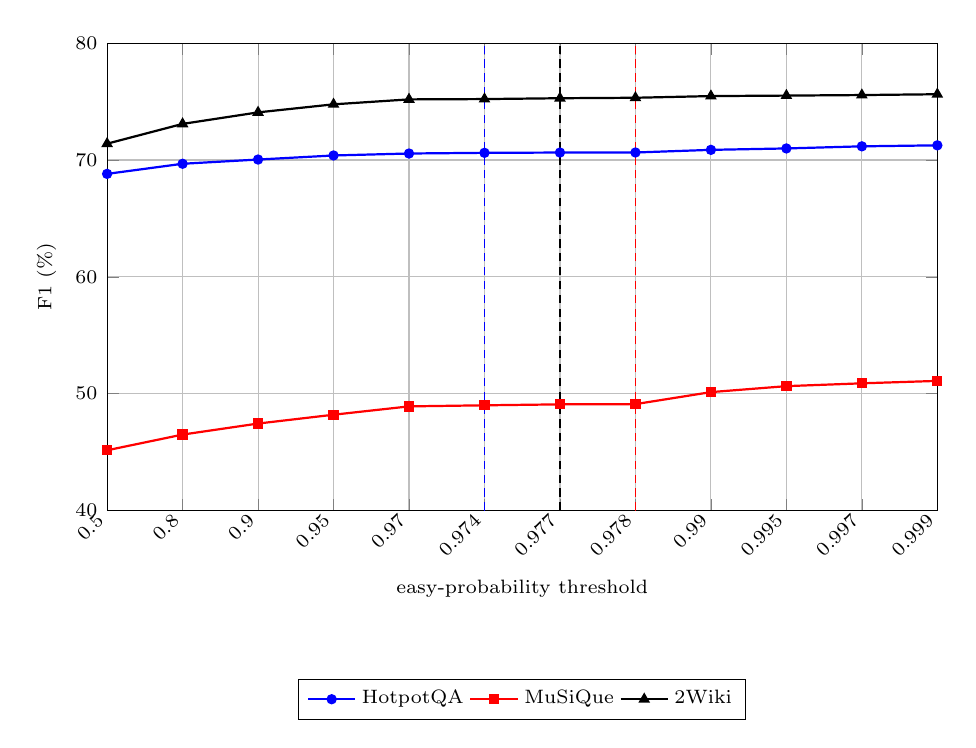
\begin{tikzpicture}
\begin{axis}[
    width=\linewidth,
    height=0.62\linewidth,
    xmin=1, xmax=12,
    ymin=40, ymax=80,
    xtick={1,2,3,4,5,6,7,8,9,10,11,12},
    xticklabels={0.5,0.8,0.9,0.95,0.97,0.974,0.977,0.978,0.99,0.995,0.997,0.999},
    xticklabel style={rotate=45,anchor=east},
    xlabel={easy-probability threshold},
    ylabel={F1 (\%)},
    grid=major,
    legend style={at={(0.5,-0.36)},anchor=north,legend columns=3,font=\scriptsize},
    tick label style={font=\scriptsize},
    label style={font=\scriptsize}
]
\addplot[blue,thick,mark=*,mark size=1.45pt] coordinates {(1,68.8116) (2,69.6764) (3,70.0387) (4,70.3858) (5,70.5543) (6,70.6131) (7,70.6367) (8,70.6410) (9,70.8671) (10,70.9876) (11,71.1689) (12,71.2531)};
\addlegendentry{HotpotQA}
\addplot[red,thick,mark=square*,mark size=1.45pt] coordinates {(1,45.1579) (2,46.5005) (3,47.4450) (4,48.2006) (5,48.9141) (6,49.0059) (7,49.0864) (8,49.1072) (9,50.1352) (10,50.6458) (11,50.8869) (12,51.0949)};
\addlegendentry{MuSiQue}
\addplot[black,thick,mark=triangle*,mark size=1.65pt] coordinates {(1,71.3944) (2,73.0880) (3,74.0745) (4,74.7631) (5,75.1856) (6,75.2130) (7,75.2852) (8,75.3249) (9,75.4695) (10,75.5102) (11,75.5570) (12,75.6269)};
\addlegendentry{2Wiki}
\addplot[blue,densely dashed,no marks] coordinates {(6,40) (6,80)};
\addplot[red,densely dashed,no marks] coordinates {(8,40) (8,80)};
\addplot[black,densely dashed,no marks] coordinates {(7,40) (7,80)};
\end{axis}
\end{tikzpicture}
\end{subfigure}
\hfill
\begin{subfigure}[b]{0.48\textwidth}
\centering
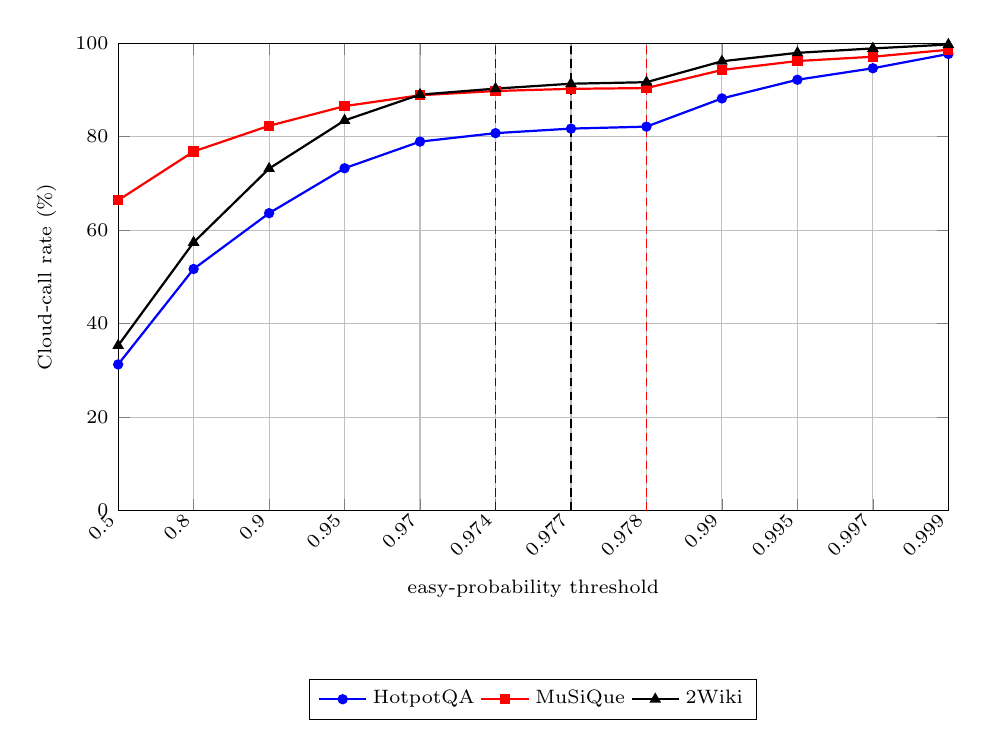
\begin{tikzpicture}
\begin{axis}[
    width=\linewidth,
    height=0.62\linewidth,
    xmin=1, xmax=12,
    ymin=0, ymax=100,
    xtick={1,2,3,4,5,6,7,8,9,10,11,12},
    xticklabels={0.5,0.8,0.9,0.95,0.97,0.974,0.977,0.978,0.99,0.995,0.997,0.999},
    xticklabel style={rotate=45,anchor=east},
    xlabel={easy-probability threshold},
    ylabel={Cloud-call rate (\%)},
    grid=major,
    legend style={at={(0.5,-0.36)},anchor=north,legend columns=3,font=\scriptsize},
    tick label style={font=\scriptsize},
    label style={font=\scriptsize}
]
\addplot[blue,thick,mark=*,mark size=1.45pt] coordinates {(1,31.2627) (2,51.6813) (3,63.6192) (4,73.2343) (5,78.9332) (6,80.7427) (7,81.7151) (8,82.1337) (9,88.1702) (10,92.1675) (11,94.6253) (12,97.6772)};
\addlegendentry{HotpotQA}
\addplot[red,thick,mark=square*,mark size=1.45pt] coordinates {(1,66.3754) (2,76.8206) (3,82.3138) (4,86.5169) (5,88.8473) (6,89.7628) (7,90.2206) (8,90.3870) (9,94.2572) (10,96.1715) (11,97.0870) (12,98.5851)};
\addlegendentry{MuSiQue}
\addplot[black,thick,mark=triangle*,mark size=1.65pt] coordinates {(1,35.3053) (2,57.3712) (3,73.1552) (4,83.4606) (5,88.9870) (6,90.2672) (7,91.3168) (8,91.6428) (9,96.1196) (10,97.9246) (11,98.8709) (12,99.6978)};
\addlegendentry{2Wiki}
\addplot[blue,densely dashed,no marks] coordinates {(6,0) (6,100)};
\addplot[red,densely dashed,no marks] coordinates {(8,0) (8,100)};
\addplot[black,densely dashed,no marks] coordinates {(7,0) (7,100)};
\end{axis}
\end{tikzpicture}
\end{subfigure}
\caption{Threshold sensitivity of CALIPER+clf: F1 (left) and cloud-call rate (right). Each marker is one measured threshold setting; lines connect adjacent measured settings for visual guidance only and do not imply measurements at intermediate thresholds. Thresholds are equally spaced categorical settings, and colored dashed lines mark the dataset-specific frozen thresholds 0.974 (HotpotQA), 0.978 (MuSiQue), and 0.977 (2Wiki).}
\label{clf_sensitivity}
\end{figure*}

\Needspace{12\baselineskip}
\subsection{Retrieval-Only Comparison}
Table~\ref{retrieval} examines the evidence supplied by the retrieval configurations before generation. CALIPER's source-routed retrieval has higher mean recall than merged training on HotpotQA and 2Wiki, supporting source-specific model selection on those sources. On MuSiQue, it has higher mean recall than BASE at every cutoff but remains below merged training. The result makes the role of retrieval adaptation source-dependent: selecting a specialist can help, but specialization is not a uniform improvement over a shared model.

\begin{table}[pos=!htb]
\caption{Retrieval-only comparison: mean evidence recall at the top 3/5/10 sentence-level units. MuSiQue maps these units to source paragraphs for recall scoring only; FT-SEP is the source-known reference.}
\label{retrieval}
\centering
\fontsize{8}{10}\selectfont
\setlength{\tabcolsep}{2.5pt}
\resizebox{\linewidth}{!}{%
\begin{tabular}{lccc}
\toprule
\textbf{Retriever} & \textbf{HotpotQA} & \textbf{MuSiQue} & \textbf{2Wiki} \\
\midrule
BASE & 70.24/80.15/89.61 & 66.96/75.14/83.91 & 62.62/72.01/85.42 \\
FT-SEP & 80.82/89.91/96.32 & 69.16/78.05/86.94 & 89.37/98.05/99.47 \\
FT-MER & 73.29/83.80/93.47 & 72.02/81.19/90.37 & 84.50/95.10/98.84 \\
CALIPER (routed) & 80.43/89.53/96.06 & 67.39/76.57/87.19 & 89.32/98.02/99.43 \\
\bottomrule
\end{tabular}}
\end{table}

Routed results on HotpotQA and 2Wiki remain below the source-known specialized reference, reflecting the difference between predicting a source and providing it directly. On MuSiQue, the specialized reference and routed system use checkpoints with different training-data organizations, so they are not a routing-only contrast.

Table~\ref{retrieval} compares retrieval-system configurations, not a single-factor routing ablation or the full generation context with its additional evidence stream.

\subsection{Qualitative Case Analysis}
Three MuSiQue examples are selected by a predetermined rule to examine collaborative answering, evidence inconsistency, and execution misrouting. The selection rule is retained in Section~8.3 of the Supplementary Configuration Notes; evidence is summarized below.

\textbf{Relation interpretation in collaborative answering.} The question ``In 2002, what company merged with the top PC manufacturer from 1994?'' requires identifying Compaq and then the other company involved in the merger. The retained records place the relevant merger sentence first in both retrieval streams. Strict Naive RAG answers \textit{Compaq}, confusing the given entity with the requested one; CALIPER returns the gold answer, \textit{Hewlett Packard}. This example illustrates a successful relation-interpretation outcome under the collaborative workflow, although the contribution of individual components cannot be isolated.

\textbf{Evidence association and benchmark scoring.} For ``When did the state where Copake Lake is located reinstate the death penalty?'', the retrieved evidence locates Copake Lake in New York, but the sentence containing the gold year, \textit{1984}, describes Oregon. Strict Naive RAG returns 1984, whereas CALIPER declines to infer a definite year and therefore misses the benchmark answer. The presence of a year in the context does not by itself support an answer: it must also refer to the entity asked about.

\textbf{Answer loss from execution misrouting.} For the MuSiQue question ``Who did the performer of Night Rocker play on Young and Restless?'', the gold answer is \textit{Snapper Foster}. The overlap-free execution classifier assigns an easy probability of 0.997155, above the frozen MuSiQue threshold of 0.978, and selects the local-only path. That path declines to answer, whereas CALIPER's collaborative output returns \textit{Snapper Foster}. The query is operationally hard because one of the three local labeling runs fails to recover the gold answer. This illustrates that high classifier confidence need not imply reliable local answering. Because the paths have different available contexts, the contrast does not isolate the effect of cloud guidance.

\section{Limitations and Deployment Scope}
CALIPER is a combined workflow with three responsibilities: guidance assists evidence use, retrieval adaptation changes the local evidence, and execution classification selects when to invoke collaboration. The ablations show that these benefits depend on the setting. Because the latency and main quality evaluations use different protocols, they do not establish a jointly measured quality--latency frontier.

The evaluation uses one Qwen local--cloud model pair and three Wikipedia-derived multi-hop QA datasets. Transfer to other model families or non-Wikipedia domains remains untested, and dataset identity is only a proxy for domain. Guidance is not evidence-verified by the cloud and may propagate errors when used locally; model changes may also alter its value. Operational-difficulty labels depend on the local model and prompt, so changes to question wording, prompts, or models require revalidation of the execution classifier and threshold. No lightweight-transformer classifier comparison is reported, and retrieval contrasts assess whole configurations rather than the isolated effect of source routing.

The locality boundary assumes an honest-but-curious cloud service: retrieved passages remain local, but queries and returned instructions may reveal sensitive content. Provider logging and retention, adversarial interactions, network compromise, and side channels are outside the evaluation. The architecture reduces retrieved-evidence exposure but does not establish differential privacy, cryptographic protection, or regulatory compliance.

Extending CALIPER to new domains requires adapting and maintaining specialized retrievers, collecting routing labels, and monitoring distribution shifts, rather than simply adding a source label. Unseen sources and uncertain routing may offset specialization gains. Reliable BASE fallback and calibrated abstention require deployment-specific validation and are not established by the reported comparisons. The two-model workflow also incurs compute and energy costs, but no power telemetry was collected to quantify energy use or carbon emissions. Future evaluation should prioritize cross-domain and cross-model transfer, routing under distribution shifts, and energy-aware execution.

\section*{Data and Artifact Availability}
The evaluation protocol, frozen predictions, aggregate metrics, paired-bootstrap outputs, and SHA-256 manifests are retained in the accompanying experimental archive. The accompanying Supplementary Configuration Notes identify the 2Wiki study input and its checksum-manifest locator. Code and selected implementation materials are available at \url{https://github.com/voidance13/CALIPER}. Public sharing of these experimental materials follows the journal's data and material sharing policies.

\section{Conclusion}
We present CALIPER, a collaborative local--cloud RAG framework that separates cloud question guidance from local evidence-grounded answering. The cloud uses only the question to provide guidance, while the local model combines that guidance with retrieved evidence to generate the answer. Source-adapted retrieval supplies evidence suited to the question, and an optional execution classifier bypasses collaboration for questions identified as locally answerable.

Experiments with the evaluated model pair and multi-hop QA tasks show that CALIPER improves answer quality over the local-model baseline and strict Naive RAG, narrowing the gap to the cloud reference. Under the evaluated latency protocol, it also reduces estimated answering latency relative to the two-stage cloud reasoning reference. The optional classifier reduces estimated latency further at some answer-quality cost. Together, the results support question-guided collaboration as a way to strengthen local evidence processing while keeping retrieved evidence local and controlling collaboration overhead.

\section*{Declaration of Generative AI and AI-Assisted Technologies in the Manuscript Preparation Process}
During the preparation of this manuscript, the authors used OpenAI Codex to assist with drafting and revising text, organizing content, language editing, and figure presentation. The AI-assisted material was reviewed and edited under author oversight, and the authors take full responsibility for the content of the publication.

% Do not allow deferred table* floats to cross into the bibliography, but let
% the preceding two-column text fill the current page first.
\FloatBarrier
% Keep the template's 8pt reference font; slightly tighten reference leading
% to prevent the final entry from occupying a separate, nearly empty page.
\renewcommand{\bibfont}{\fontsize{8pt}{9.5pt}\selectfont}
\bibliographystyle{model1-num-names}
% Keep each bibliography entry together within one column.  This lets the
% left column finish at an entry boundary before the right column begins.
\AtBeginEnvironment{thebibliography}{%
  \interlinepenalty=10000
  \clubpenalty=10000
  \widowpenalty=10000
}
\bibliography{references}

\end{document}
